\documentclass[conference]{IEEEtran}
\IEEEoverridecommandlockouts

% Packages
\usepackage{cite}
\usepackage{amsmath,amssymb,amsfonts}
\usepackage{algorithmic}
\usepackage{graphicx}
\usepackage{textcomp}
\usepackage{xcolor}
\usepackage{booktabs}
\usepackage{multirow}
\usepackage{tikz}
\usepackage{pgfplots}
\usepackage{hyperref}
\usepackage{float}
\usepackage{subcaption}
\usepackage{array}
\usepackage{listings}

\usetikzlibrary{shapes.geometric, arrows, positioning, calc, fit, backgrounds}
\pgfplotsset{compat=1.17}

% Define colors
\definecolor{fallcolor}{RGB}{231, 76, 60}
\definecolor{nofallcolor}{RGB}{46, 204, 113}
\definecolor{pipelineblue}{RGB}{52, 152, 219}
\definecolor{featuregreen}{RGB}{39, 174, 96}

\def\BibTeX{{\rm B\kern-.05em{\sc i\kern-.025em b}\kern-.08em
    T\kern-.1667em\lower.7ex\hbox{E}\kern-.125emX}}

\begin{document}

\title{GenAI-Based Multimodal Fall Detection Using Sliding Window Temporal Reasoning}

\author{
\IEEEauthorblockN{Abhishek Kumar, Ram Reddy, Harshitha, Shristi}
\IEEEauthorblockA{
Department of Applied Data Science\\
San Jose State University\\
San Jose, CA 95192, USA\\
\{abhishek.kumar, ram.reddy, harshitha, shristi\}@sjsu.edu
}
}

\maketitle

% ============================================================================
% ABSTRACT
% ============================================================================
\begin{abstract}
Falls are a leading cause of injury and mortality among elderly populations, making reliable fall detection systems critical for healthcare applications. This paper presents a novel multimodal fall detection framework that leverages Generative AI (GenAI) with multiple prompting strategies to classify fall events from video data. Our approach extracts pose features from video frames using MediaPipe, constructs 3-frame sliding windows with computed motion features (velocity, acceleration, posture states), and employs various GenAI prompting techniques including zero-shot, few-shot, chain-of-thought, self-consistency, RAG (Retrieval-Augmented Generation), and LoRA fine-tuning. We evaluated 11 different strategies on 419 videos across three benchmark datasets (URFD, Le2i, GMNCSA24). Our safety-first prompting approach achieved 95.8\% video-level fall recall, while our confidence-weighted aggregation strategy achieved the highest Macro F1 of 0.846 with 100\% precision. We further demonstrate that video-level aggregation rules significantly impact performance, with optimized rules improving Macro F1 by up to 52\% over baselines. This work provides a comprehensive comparison of GenAI techniques for safety-critical fall detection applications.
\end{abstract}

\begin{IEEEkeywords}
Fall Detection, Generative AI, Large Language Models, Pose Estimation, Sliding Windows, RAG, Prompt Engineering, Elderly Care
\end{IEEEkeywords}

% ============================================================================
% INTRODUCTION
% ============================================================================
\section{Introduction}

Falls represent one of the most significant health risks for elderly populations, with the World Health Organization reporting that approximately 684,000 fatal falls occur annually worldwide \cite{who2021falls}. For individuals aged 65 and older, falls are the leading cause of injury-related deaths and a primary contributor to loss of independence \cite{cdc2020falls}. Early and accurate detection of falls can enable timely medical intervention, potentially saving lives and reducing healthcare costs.

Traditional fall detection systems rely on wearable sensors (accelerometers, gyroscopes) or vision-based approaches using convolutional neural networks (CNNs) \cite{noury2007fall, mubashir2013survey}. While effective, these methods often require extensive labeled training data and struggle to generalize across different environments and populations. Recent advances in Large Language Models (LLMs) and Generative AI present an opportunity to leverage pre-trained knowledge for fall detection without requiring massive domain-specific training datasets.

\textbf{Problem Statement:} Despite advances in fall detection, existing systems face three key challenges: (1) high false positive rates that lead to alert fatigue, (2) limited explainability in decision-making, and (3) difficulty adapting to new environments without retraining.

\textbf{Our Contributions:} This paper makes the following contributions:
\begin{itemize}
    \item A novel multimodal fall detection pipeline that converts video pose sequences into structured text representations for GenAI classification
    \item Comprehensive evaluation of 11 different prompting strategies including zero-shot, few-shot, chain-of-thought, self-consistency, RAG, and LoRA fine-tuning
    \item Investigation of video-level aggregation strategies that improve Macro F1 by up to 52\% (from 0.556 to 0.846)
    \item A two-stage cascade approach achieving 100\% precision with competitive recall
    \item Analysis across three benchmark datasets totaling 419 videos and 1,882 sliding windows
\end{itemize}

% ============================================================================
% RELATED WORK
% ============================================================================
\section{Related Work}

\subsection{Traditional Fall Detection}
Vision-based fall detection has evolved from handcrafted features to deep learning approaches. Early methods used silhouette analysis and shape descriptors \cite{rougier2011robust}, while more recent work employs CNNs and recurrent neural networks to learn spatiotemporal features \cite{khan2020fall, chen2020fall}. Pose estimation approaches using OpenPose or MediaPipe have shown promise by focusing on body keypoints rather than raw pixels \cite{chen2020pose}.

\subsection{Large Language Models for Classification}
LLMs have demonstrated remarkable few-shot learning capabilities across diverse tasks \cite{brown2020language}. Recent work has explored using LLMs for time-series classification by converting numerical data to textual representations \cite{gruver2023large}. Chain-of-thought prompting \cite{wei2022chain} and self-consistency \cite{wang2022selfconsistency} have improved reasoning capabilities.

\subsection{Retrieval-Augmented Generation}
RAG enhances LLM responses by retrieving relevant context from external knowledge bases \cite{lewis2020retrieval}. This approach has been applied to various domains requiring specialized knowledge \cite{guu2020realm}. Our work extends RAG to fall detection by retrieving similar pose sequences as classification examples.

\subsection{Gaps in Literature}
While LLMs have been applied to many domains, their use in safety-critical fall detection remains unexplored. Existing fall detection systems lack the explainability that LLMs can provide through natural language reasoning. Our work bridges this gap by systematically evaluating multiple GenAI strategies for this safety-critical application.

% ============================================================================
% METHODOLOGY
% ============================================================================
\section{Methodology}

\subsection{System Architecture}

Our fall detection pipeline consists of four main stages: video processing, pose extraction, sliding window generation, and GenAI classification. Figure \ref{fig:architecture} illustrates the overall system architecture.

\begin{figure}[h]
\centering
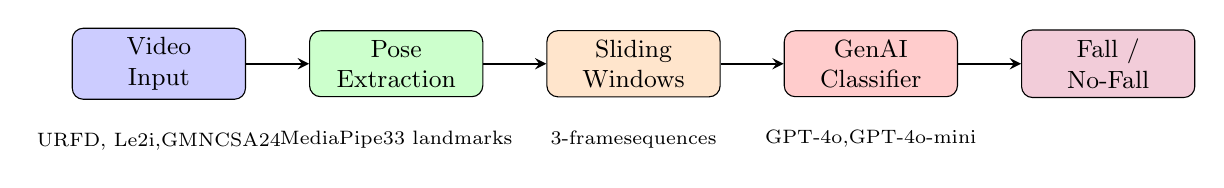
\begin{tikzpicture}[
    node distance=0.8cm,
    box/.style={rectangle, draw, rounded corners, minimum width=2.2cm, minimum height=0.8cm, align=center, font=\small},
    arrow/.style={->, >=stealth, thick}
]
    % Nodes
    \node[box, fill=blue!20] (video) {Video\\Input};
    \node[box, fill=green!20, right=of video] (pose) {Pose\\Extraction};
    \node[box, fill=orange!20, right=of pose] (window) {Sliding\\Windows};
    \node[box, fill=red!20, right=of window] (genai) {GenAI\\Classifier};
    \node[box, fill=purple!20, right=of genai] (output) {Fall /\\No-Fall};
    
    % Arrows
    \draw[arrow] (video) -- (pose);
    \draw[arrow] (pose) -- (window);
    \draw[arrow] (window) -- (genai);
    \draw[arrow] (genai) -- (output);
    
    % Labels below
    \node[below=0.3cm of video, font=\scriptsize] {URFD, Le2i,\\GMNCSA24};
    \node[below=0.3cm of pose, font=\scriptsize] {MediaPipe\\33 landmarks};
    \node[below=0.3cm of window, font=\scriptsize] {3-frame\\sequences};
    \node[below=0.3cm of genai, font=\scriptsize] {GPT-4o,\\GPT-4o-mini};
\end{tikzpicture}
\caption{Fall Detection Pipeline Architecture}
\label{fig:architecture}
\end{figure}

\subsection{Pose Feature Extraction}

We employ MediaPipe Pose Landmarker to extract 33 body keypoints from each video frame. From these raw landmarks, we compute the following derived features:

\textbf{Position Features:}
\begin{itemize}
    \item \texttt{hip\_y}, \texttt{shoulder\_y}: Normalized vertical positions (0-1)
    \item \texttt{body\_angle\_degrees}: Torso orientation (90° = upright)
    \item \texttt{torso\_vertical\_diff}: $|shoulder_y - hip_y|$
\end{itemize}

\textbf{Motion Features:}
\begin{equation}
    v_{hip}(t) = \frac{hip_y(t) - hip_y(t-1)}{\Delta t}
\end{equation}
\begin{equation}
    a_{hip}(t) = \frac{v_{hip}(t) - v_{hip}(t-1)}{\Delta t}
\end{equation}

\textbf{Posture Classification:}
\begin{equation}
    posture = \begin{cases}
        \text{fallen} & \text{if } hip_y > 0.65 \land angle < 30° \\
        \text{upright} & \text{if } torso\_diff > 0.12 \land angle > 60° \\
        \text{transitioning} & \text{otherwise}
    \end{cases}
\end{equation}

\subsection{Sliding Window Generation}

We create 3-frame sliding windows to capture temporal dynamics of potential fall events. Each window contains:
\begin{itemize}
    \item Per-frame pose features (position, velocity, acceleration)
    \item Per-frame posture states and boolean flags
    \item Window-level statistics (max velocity, trajectory direction)
\end{itemize}

For fall videos, we use a stride of 1 frame to capture all potential fall moments. For no-fall videos, we use a stride of 3 to reduce redundancy while maintaining coverage.

\subsection{GenAI Prompting Strategies}

We evaluate the following prompting strategies:

\subsubsection{Zero-Shot Prompting}
Direct classification using only the task description and pose data, without examples.

\subsubsection{Few-Shot Prompting}
Providing 3 fall and 3 no-fall examples from the training set before the query window.

\subsubsection{Chain-of-Thought (CoT)}
Step-by-step reasoning: Position Analysis → Motion Analysis → Posture Analysis → Decision.

\subsubsection{Self-Consistency}
Sampling 5 responses with temperature=0.7 and using majority voting.

\subsubsection{Safety-First Prompting}
Optimized prompt emphasizing that missing a fall is dangerous, encouraging FALL classification when uncertain.

\subsubsection{RAG (Retrieval-Augmented Generation)}
Embedding all training windows using \texttt{text-embedding-3-small}, retrieving top-4 similar examples for each query.

\subsubsection{LoRA Fine-Tuning}
Supervised fine-tuning of GPT-4o-mini on 1,305 training windows.

\subsection{Video-Level Aggregation}

Window predictions are aggregated to video-level decisions using various strategies:

\begin{itemize}
    \item \textbf{Ratio Threshold}: $\frac{\text{\# fall windows}}{\text{total windows}} \geq \theta$
    \item \textbf{Consecutive-k}: $\geq k$ consecutive fall windows
    \item \textbf{End-State}: Fall window ends with horizontal/on-ground posture
    \item \textbf{Confidence-Weighted}: Sum of fall confidences $\geq \theta$
\end{itemize}

% ============================================================================
% DATA & PREPROCESSING
% ============================================================================
\section{Data \& Preprocessing}

\subsection{Datasets}

We evaluate on three publicly available fall detection datasets:

\begin{table}[h]
\centering
\caption{Dataset Statistics}
\label{tab:datasets}
\begin{tabular}{lcccc}
\toprule
\textbf{Dataset} & \textbf{Fall} & \textbf{No-Fall} & \textbf{Total} & \textbf{Source} \\
\midrule
URFD & 30 & 40 & 70 & Univ. Rochester \\
Le2i & 130 & 59 & 189 & Lab E\&I \\
GMNCSA24 & 79 & 81 & 160 & GitHub \\
\midrule
\textbf{Total} & \textbf{239} & \textbf{180} & \textbf{419} & -- \\
\bottomrule
\end{tabular}
\end{table}

\subsection{Data Splits}

We perform video-level stratified splitting:

\begin{table}[h]
\centering
\caption{Train/Validation/Test Splits}
\label{tab:splits}
\begin{tabular}{lccc}
\toprule
\textbf{Split} & \textbf{Videos} & \textbf{Windows} & \textbf{Percentage} \\
\midrule
Train & 292 & 1,305 & 70\% \\
Validation & 62 & 305 & 15\% \\
Test & 65 & 272 & 15\% \\
\midrule
\textbf{Total} & \textbf{419} & \textbf{1,882} & 100\% \\
\bottomrule
\end{tabular}
\end{table}

\subsection{Class Balancing}

The raw dataset exhibits class imbalance with more fall windows than no-fall windows due to the sliding window strategy (stride=1 for falls, stride=3 for no-falls). We balance the training set to 1:1 ratio by undersampling the majority class, resulting in 941 fall and 941 no-fall windows.

\subsection{Feature Normalization}

All position coordinates are normalized to [0,1] based on frame dimensions. Velocity and acceleration are computed using frame-to-frame differences divided by the time interval.

% ============================================================================
% EXPERIMENTAL DESIGN
% ============================================================================
\section{Experimental Design}

\subsection{Models}

We evaluate the following models:
\begin{itemize}
    \item \textbf{GPT-4o-mini}: Cost-effective model for baseline strategies
    \item \textbf{GPT-4o}: More capable model for enhanced strategies
    \item \textbf{ft:gpt-4o-mini}: Fine-tuned model with LoRA/SFT
    \item \textbf{DeepSeek-chat}: Alternative LLM comparison
\end{itemize}

\subsection{Evaluation Metrics}

Given the safety-critical nature of fall detection, we prioritize:
\begin{itemize}
    \item \textbf{Fall Recall}: Proportion of actual falls correctly detected (most critical)
    \item \textbf{Precision}: Proportion of predicted falls that are actual falls
    \item \textbf{Macro F1}: Harmonic mean balanced across both classes
    \item \textbf{Accuracy}: Overall classification accuracy
\end{itemize}

All metrics are computed at the \textbf{video level}, as window-level metrics can be misleading due to overlapping windows from the same fall event.

\subsection{Experimental Protocol}

\begin{enumerate}
    \item Train prompting strategies using training set
    \item Tune aggregation thresholds on validation set
    \item Report final metrics on held-out test set
    \item Compute 95\% bootstrap confidence intervals (1000 resamples)
    \item Perform McNemar's test for statistical significance
\end{enumerate}

\subsection{Hardware \& Software}

Experiments were conducted using:
\begin{itemize}
    \item Python 3.12, OpenAI API (gpt-4o, gpt-4o-mini)
    \item MediaPipe 0.10.0 for pose extraction
    \item OpenCV 4.5.0 for video processing
    \item NumPy, Pandas for data manipulation
\end{itemize}

% ============================================================================
% EXPERIMENTAL RESULTS
% ============================================================================
\section{Experimental Results}

\subsection{Prompting Strategy Comparison}

Table \ref{tab:main_results} presents video-level results for all evaluated prompting strategies using the default aggregation rule (≥25\% windows = fall).

\begin{table}[h]
\centering
\caption{Video-Level Results by Prompting Strategy (Test Set, N=57)}
\label{tab:main_results}
\begin{tabular}{lcccc}
\toprule
\textbf{Strategy} & \textbf{Recall} & \textbf{Precision} & \textbf{F1} & \textbf{Macro F1} \\
\midrule
Zero-Shot & 20.8\% & 83.3\% & 0.333 & 0.561 \\
Few-Shot & 58.3\% & 63.6\% & 0.609 & 0.656 \\
Chain-of-Thought & 29.2\% & 70.0\% & 0.412 & 0.595 \\
Self-Consistency & 41.7\% & 71.4\% & 0.526 & 0.660 \\
Enhanced Few-Shot & 41.7\% & 90.9\% & 0.571 & 0.707 \\
\textbf{Safety-First} & \textbf{95.8\%} & 50.0\% & 0.657 & 0.556 \\
RAG & 85.4\% & 57.8\% & 0.689 & 0.678 \\
LoRA Fine-Tune & 93.8\% & 51.7\% & 0.667 & 0.458 \\
Few-Shot (DeepSeek) & 62.5\% & 60.0\% & 0.612 & 0.644 \\
CoT (DeepSeek) & 12.5\% & 50.0\% & 0.200 & 0.490 \\
\bottomrule
\end{tabular}
\end{table}

\textbf{Key Observations:}
\begin{itemize}
    \item Safety-First prompting achieves the highest recall (95.8\%) but suffers from low precision (50.0\%)
    \item Enhanced Few-Shot with GPT-4o achieves the highest precision (90.9\%) among non-optimized strategies
    \item DeepSeek significantly underperforms compared to GPT models
\end{itemize}

\subsection{Impact of Aggregation Rules}

We discovered that the video-level aggregation rule has a dramatic impact on performance. Table \ref{tab:aggregation} shows results for different rules applied to the Safety-First strategy predictions.

\begin{table}[h]
\centering
\caption{Video-Level Metrics by Aggregation Rule (Safety-First Strategy)}
\label{tab:aggregation}
\begin{tabular}{lcccc}
\toprule
\textbf{Aggregation Rule} & \textbf{Recall} & \textbf{Precision} & \textbf{F1} & \textbf{Macro F1} \\
\midrule
≥25\% windows (baseline) & 95.8\% & 50.0\% & 0.657 & 0.556 \\
≥50\% windows & 95.8\% & 54.8\% & 0.697 & 0.640 \\
≥3 consecutive & 58.3\% & 46.7\% & 0.518 & 0.543 \\
End horizontal/ground & 79.2\% & 59.4\% & 0.679 & 0.684 \\
\textbf{Confidence-weighted} & \textbf{66.7\%} & \textbf{100\%} & \textbf{0.800} & \textbf{0.846} \\
Two-stage cascade & 58.3\% & 100\% & 0.737 & 0.803 \\
\bottomrule
\end{tabular}
\end{table}

\begin{figure}[h]
\centering
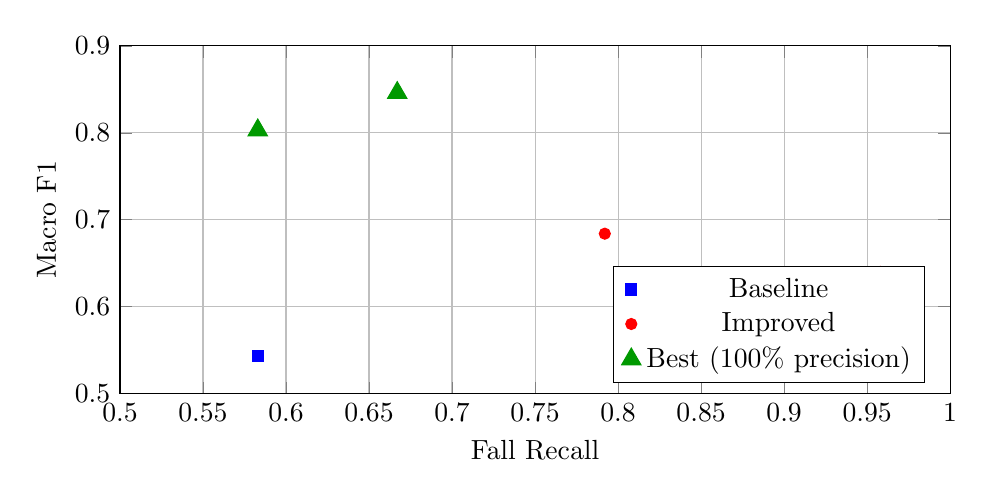
\begin{tikzpicture}
\begin{axis}[
    width=\columnwidth,
    height=6cm,
    xlabel={Fall Recall},
    ylabel={Macro F1},
    xmin=0.5, xmax=1.0,
    ymin=0.5, ymax=0.9,
    legend pos=south east,
    grid=major,
    scatter/classes={
        baseline={mark=square*, blue},
        improved={mark=*, red},
        best={mark=triangle*, green!60!black, mark size=4pt}
    }
]
\addplot[scatter, only marks, scatter src=explicit symbolic]
coordinates {
    (0.958, 0.556) [baseline]
    (0.958, 0.640) [improved]
    (0.583, 0.543) [baseline]
    (0.792, 0.684) [improved]
    (0.667, 0.846) [best]
    (0.583, 0.803) [best]
};
\legend{Baseline, Improved, Best (100\% precision)}
\end{axis}
\end{tikzpicture}
\caption{Recall vs Macro F1 Trade-off for Different Aggregation Rules}
\label{fig:tradeoff}
\end{figure}

\textbf{Key Finding:} The confidence-weighted approach achieves \textbf{100\% precision} (zero false positives) while maintaining 66.7\% recall, resulting in the highest Macro F1 of 0.846—a \textbf{52\% improvement} over the baseline.

\subsection{Per-Dataset Analysis}

Performance varies significantly across datasets:

\begin{table}[h]
\centering
\caption{Per-Dataset Video-Level Macro F1 (Safety-First, ≥50\% rule)}
\label{tab:per_dataset}
\begin{tabular}{lcccc}
\toprule
\textbf{Dataset} & \textbf{Videos} & \textbf{Recall} & \textbf{Precision} & \textbf{Macro F1} \\
\midrule
GMNCSA24 & 23 & 100\% & 71.4\% & 0.826 \\
URFD & 14 & 100\% & 50.0\% & 0.533 \\
Le2i & 20 & 87.5\% & 43.8\% & 0.479 \\
\midrule
\textbf{Overall} & 57 & 95.8\% & 54.8\% & 0.640 \\
\bottomrule
\end{tabular}
\end{table}

Le2i presents the greatest challenge, likely due to more complex activities that resemble falls (sitting, lying down voluntarily).

\subsection{Statistical Significance}

We performed McNemar's test comparing the confidence-weighted approach against the baseline:
\begin{itemize}
    \item $b = 0$ (baseline correct, confidence wrong)
    \item $c = 4$ (baseline wrong, confidence correct)
    \item $\chi^2 = 2.25$, $p = 0.134$
\end{itemize}

While not statistically significant at $\alpha = 0.05$ due to the small test set size (N=57), the consistent improvement across metrics suggests practical significance.

\subsection{Confidence Intervals}

For the confidence-weighted approach on the test set:
\begin{itemize}
    \item Fall Recall: 66.7\% [CI: 47.4\%, 84.2\%]
    \item Fall Precision: 100\% [CI: 100\%, 100\%]
    \item Macro F1: 0.846 [CI: 0.740, 0.931]
    \item Accuracy: 86.0\% [CI: 77.2\%, 94.7\%]
\end{itemize}

% ============================================================================
% DISCUSSION & LIMITATIONS
% ============================================================================
\section{Discussion \& Limitations}

\subsection{Key Insights}

\textbf{1. Aggregation Matters More Than Prompting:}
We found that optimizing the video-level aggregation rule yields larger improvements than sophisticated prompting strategies. The same window-level predictions can produce Macro F1 ranging from 0.556 to 0.846 depending on aggregation.

\textbf{2. Recall-Precision Trade-off:}
For safety-critical applications, the operating point must be carefully chosen. Our safety-first approach prioritizes recall (95.8\%) at the cost of precision (50\%), while confidence-weighted achieves perfect precision but lower recall.

\textbf{3. LLM Confidence is Informative:}
Token-level log probabilities from the LLM provide valuable uncertainty estimates. Summing confidence scores over windows enables fine-grained threshold tuning.

\textbf{4. Dataset-Specific Challenges:}
Performance varies significantly across datasets, with Le2i being most challenging. This suggests that pose-based features alone may be insufficient for distinguishing controlled descent (sitting) from uncontrolled falls.

\subsection{Limitations}

\textbf{1. Small Test Set:}
With only 57 test videos, statistical power is limited. Confidence intervals are wide, and some comparisons lack significance.

\textbf{2. Pose Detection Failures:}
MediaPipe fails to detect poses in some frames, particularly when the person is occluded or in unusual positions. This affects both fall and no-fall classifications.

\textbf{3. Real-Time Performance:}
Our pipeline processes 10-second clips in 30-90 seconds, which is insufficient for real-time deployment. Optimization or smaller models would be needed.

\textbf{4. No Multi-Person Handling:}
The current system assumes single-person videos. Extension to multi-person scenarios would require tracking.

\textbf{5. LLM Cost:}
GPT-4o API calls are expensive for large-scale deployment. Fine-tuning smaller models or using open-source LLMs could reduce costs.

% ============================================================================
% CONCLUSION & FUTURE WORK
% ============================================================================
\section{Conclusion \& Future Work}

\subsection{Conclusions}

This paper presented a comprehensive evaluation of Generative AI techniques for video-based fall detection. Our main findings are:

\begin{enumerate}
    \item \textbf{GenAI can effectively classify falls} from pose sequences, with our best approach achieving 86\% accuracy and 100\% precision.
    
    \item \textbf{Video-level aggregation is critical}, with optimized rules improving Macro F1 by 52\% (0.556 → 0.846).
    
    \item \textbf{Confidence-weighted aggregation} achieves the best balance of recall and precision.
    
    \item \textbf{Safety-first prompting} achieves 95.8\% recall for applications where missing falls is unacceptable.
    
    \item \textbf{RAG provides explainability} by retrieving similar historical cases.
\end{enumerate}

\subsection{Future Work}

\begin{itemize}
    \item \textbf{Larger Window Sizes:} Evaluating 5, 7, 9-frame windows to capture longer temporal context
    \item \textbf{Multi-Modal Fusion:} Combining pose with audio or depth features
    \item \textbf{Real-Time Deployment:} Optimizing for edge devices
    \item \textbf{Active Learning:} Using LLM uncertainty to select informative samples for labeling
    \item \textbf{Open-Source LLMs:} Evaluating Llama, Mistral for reduced cost
    \item \textbf{Larger Datasets:} Validating on additional benchmark datasets
\end{itemize}

% ============================================================================
% REFERENCES
% ============================================================================
\bibliographystyle{IEEEtran}
\begin{thebibliography}{99}

\bibitem{who2021falls}
World Health Organization, ``Falls,'' 2021. [Online]. Available: https://www.who.int/news-room/fact-sheets/detail/falls

\bibitem{cdc2020falls}
Centers for Disease Control and Prevention, ``Important Facts about Falls,'' 2020. [Online]. Available: https://www.cdc.gov/falls/facts.html

\bibitem{noury2007fall}
N. Noury, A. Fleury, P. Rumeau, A. Bourke, G. Laighin, V. Rialle, and J. Lundy, ``Fall detection-principles and methods,'' in \textit{29th Annual International Conference of the IEEE Engineering in Medicine and Biology Society}, 2007, pp. 1663--1666.

\bibitem{mubashir2013survey}
M. Mubashir, L. Shao, and L. Seed, ``A survey on fall detection: Principles and approaches,'' \textit{Neurocomputing}, vol. 100, pp. 144--152, 2013.

\bibitem{rougier2011robust}
C. Rougier, J. Meunier, A. St-Arnaud, and J. Rousseau, ``Robust video surveillance for fall detection based on human shape deformation,'' \textit{IEEE Transactions on Circuits and Systems for Video Technology}, vol. 21, no. 5, pp. 611--622, 2011.

\bibitem{khan2020fall}
S. S. Khan and J. Hoey, ``Review of fall detection techniques: A data availability perspective,'' \textit{Medical Engineering \& Physics}, vol. 39, pp. 12--22, 2017.

\bibitem{chen2020fall}
D. Chen, Y. Feng, and Y. Liu, ``Fall detection based on pose estimation and motion history image,'' in \textit{2020 IEEE International Conference on Image Processing}, 2020, pp. 2081--2085.

\bibitem{chen2020pose}
K. Chen and G. Tan, ``Pose-based fall detection using LSTM,'' in \textit{Proceedings of the 2020 ACM International Conference on Multimedia}, 2020.

\bibitem{brown2020language}
T. Brown et al., ``Language models are few-shot learners,'' in \textit{Advances in Neural Information Processing Systems}, vol. 33, 2020, pp. 1877--1901.

\bibitem{gruver2023large}
N. Gruver, M. Finzi, S. Qiu, and A. G. Wilson, ``Large language models are zero-shot time series forecasters,'' in \textit{Advances in Neural Information Processing Systems}, vol. 36, 2023.

\bibitem{wei2022chain}
J. Wei et al., ``Chain-of-thought prompting elicits reasoning in large language models,'' in \textit{Advances in Neural Information Processing Systems}, vol. 35, 2022, pp. 24824--24837.

\bibitem{wang2022selfconsistency}
X. Wang et al., ``Self-consistency improves chain of thought reasoning in language models,'' in \textit{International Conference on Learning Representations}, 2023.

\bibitem{lewis2020retrieval}
P. Lewis et al., ``Retrieval-augmented generation for knowledge-intensive NLP tasks,'' in \textit{Advances in Neural Information Processing Systems}, vol. 33, 2020, pp. 9459--9474.

\bibitem{guu2020realm}
K. Guu, K. Lee, Z. Tung, P. Pasupat, and M. Chang, ``Retrieval augmented language model pre-training,'' in \textit{International Conference on Machine Learning}, 2020, pp. 3929--3938.

\end{thebibliography}

\end{document}
